\chapter{Synthedemic Modelling}
\label{ch:multi}
The classic epidemic model brings to mind images of a single curve
with a single peak. When measuring the spread of a single infectious
disease within a closed population, this is often a realistic
characterisation. For example, the number of people in London infected
with a new strain of flu virus might resemble this curve. 

Recent work has highlighted the limitations of the single epidemic
based approach in characterising certain epidemic phenomena, particulary with
regards to viral internet trends.\cite{marily2013, marily2014} A
recent adaptation of the field of \emph{synepidemiology} termed
\emph{synthemics} has been proposed as a potential avenue of further
research. The key challenges of the synthedemic modelling procedure are to
identify the number of underlying epidemics, to identify when these
sub epidemics start, and to identify the type of epidemic model that
best describes each sub epidemic. Furthermore, as the number of
included sub epidemics increases, so to do the number of parameters to
be optimised the corresponding parameter search space. 

In this section we discuss an implementation that aims to address these challenges,
and the particular problems and solutions that arise during the course
of the project.


\section{Identifying Sub Epidemic Start Time}
In the single epidemic fitting framework, it is assumed that there is
only one epidemic in the dataset, and that it can be considered to
have started right at the beginning of the dataset. However, when
considering multiple epidemics simultaneously, it is not possible to
make this assumption, as multiple sub epidemics might start and finish during
the iterative fitting procedure. Furthermore, when multiple epidemics
are progressing simultaneously, it might not be possible to detect the
start of a new epidemic until it is well underway. The start time of
the epidemic therefore might (and probably will not) match the
detection time. The first step in developing a
synthedemic model fitting framework is therefore to implement a means
to detect and record epidemic start times, and to consider how these
start times will be included in the optimisation procedure.



\subsection{Epidemic Detection}
The aim of detecting an epidemic outbreak is to determine when the
level of infected individuals has begun to rise above the expected
baseline level. In most cases, there will be a certain number of
background infecteds that are endemic in the population. For example,
consider that there will be some individuals infected with flu
throughout the year. The first step in our detection procedure is
therefore to establish a baseline level, taken as the mean of the data
points up until detection.

At each time point, residuals are generated from the difference
between the current best fitting model and the available data. If
there are no active epidemics, the best fitting model is taken as the
baseline level. We then check the latest residual for signs of an
epidemic outbreak. If the latest residual lies a certain number of
standard deviations away from the mean of the previous residuals, then
we suspect that an outbreak might have occured. As the detection
procedure is dependent on the variation in the past residuals, the sensitivity of
outbreak detection is dependent on the noise of the data itself. If
the data set shows very low variation, then the standard deviation of
the residuals will be low; resulting in a low detection
threshold. Similarly, if the standard deviation is very high (as might
be the case with real world data), then the threshold will be very
high. In terms of implementation, we therefore couple the residual
detection threshold with a measure of the current model fit. If the
current model fit is less than a certain value, then the model fit has
deteriorated sufficiently to consider the addition of another sub
epidemic.

Although the above detection method is a sound heuristic approach, the
dependence on the quality of the data means that detection time may
be inaccurate. When the outbreak begins gradually, the change to the
mean and standard deviation of the residuals may be small enough that
the latest residual is never outside of the detection
range. In epidemic outbreaks of infectious diseases, proxies for
detection might be used in place of analysing the epidemic data
itself. Please refer to section EVALUATION for further discussion of
alternative approaches to outbreak detection.


 For example, the World Health Organisation gathers reports and
rumours of suspected outbreaks from various informal sources and
national health organisations in the hopes of
investigating and catching a potential outbreak as early as
possible. CITE WHO. One tool used by the WHO is the Global Public
Health Intelligence Network



\subsection{Optimising Epidemic Start Times}
Once an epidemic outbreak has been detected, the next challenge is to
find the actual start time of the epidemic. Simply using the detection
time of the sub epidemic as the actual start time is unsatisfactory,
as it assumes that the detection procedure will pick up a new outbreak
as soon as it starts. Some sub epidemics will be hidden within larger
outbreaks and may not be detected until well into their course. 

An initial naive approach to finding the start time of each sub
epidemic might be to consider each possible combination of epidemic
start times. If we consider every possible start time, this would
result in \emph{n}
optimisations for a single epidemic, where \emph{n} is the number of
data points currently available. As soon as multiple epidemics are
considered simultaneously, this quickly becomes infeasible as the
complexity increases with the number of sub epidemics. An heuristic adaption to this is to only consider a subset of start
time combinations. For example, we can consider only the start times
within a window of the detection time, and assume that the ordering of
start times does not matter. This results in \emph{tCn} combinations
of start times, where \emph{t} is the number of time points under
consideration, and \emph{n} is the number of epidemics to be
fit. 

Although such heuristics  might provide a
conceptually simple optimisation approach, they avoid the problem of
including $t_0$ in the optimisation procedure directly. Doing should
allows for the start time of each sub epidemic to be found
precisely. Furthermore, doing so allows us to consider the start time
as a continuous variable, making the model fit much more accurate. We
therefore chose to initially include $t_0$ as an unknown parameter in
the optimisation procedure. Giving the Nelder Mead algorithm a
completely random time as a seed value risks producing an extremely
high initial SSE value. We therefore use the detection time minus a
small value (to account for delayed detection) of the epidemic
as the seed value for the optimisation procedure. 

\section{Initial Approach}
The initial approach aims to iterate over a set of epidemic data,
where it is not assumed that there is an ongoing epidemic from the
start. We include the transition parameters, beta and gamma, as well
as S0 and t0 in the optimisation procedure. As in the single fitting
framework, at each time point we produce random seed values and choose
the best run from ten independent as the best fitting model. T0 is
seeded as the detection time of the epidemic. We first fit the
currently known \emph{k} epidemics, and then consider the addition of
an epidemic when the model fit has deteriorated sufficiently and
the latest residual is a certain number of standard deviations away
from the previous residuals' mean. By only adding an additional
epidemic when the model fit has deteriorated sufficiently, we avoid
needlessly overfitting the data when an outlying data point might
falsly suggest the start of a new epidemic.

We initially consider only SIR models, which result in a combined
parameter set of $(\beta^{(k)},\gamma^{(k)},\S_{0}^{(k)},t_0^{(k)})$ to
be optimised. One risk of only considering the addition of epidemics
is that we risk overfitting the data. To avoid this, we also consider the removal of a
sub epidemic at each time point. This is done by removing each sub
epidemic from the current set in turn and reoptimising the remaining
model. If this fit of $k-1$ epidemics is sufficient, we
permanently remove the epidemic from the list.

\subsection{Practicality Considerations}
As the fitting process is a computationally time intensive procedure,
we adhere to the following heuristics to prevent the run time from
becoming infeasible:

\begin{enumerate}
\item Only one epidemic is added or removed at each stage.
\item For SIR epidemics (and sub types in later implementations) we assume that the number if initial infected
  individuals is 1. 
\item For EXP epidemics, the number of infected individuals is
  included as an unknown parameter. A potential simplification of this
  is to use the difference between the current best fitting model and
  the time point at which the epidemic is detected. However, this
  does not allow for the possibility that our current best fitting
  model might not be optimal.
\item The seed time for $t_0$ for SIR type epidemics is taken as the
  detection time minus 10, and searched within the range
  $t-50\leftarrow t$, where $t$ is the detection time.
\item At each time point, we choose the best of 10 independent
  optimisation runs for $k$ epidemics and $k-1$ epidemics, testing the
  removal of all current epidemics to prevent overfitting. When adding
  epidemics, we consider adding each candidate model if the latest
  residual is over three standard deviations away from the mean residual size.
\end{enumerate}

\subsection{Initial Testing}
The multiple epidemic fitting framework was firstly tested using
synthetic data generated by the \emph{GillespieSSA} algorithm in R. To
simulate multiple overlapping epidemics, we run \emph{GillespieSSA}
for each sub epidemic and offset the values by the desired $t_0$;
adding the infected values of each sub epidemic on the corresponding
time points. Two \emph{SIR} models were combined with the following
parameters:

$\beta^1=0.001, \gamma^1 = 0.1, S_0 = 500, t_0 = 10$\\
$\beta^1=0.0008, \gamma^1 = 0.008, S_0 = 800, t_0 = 30$

The initial implementation detected the start of the first epidemic at
$t = 14$, and proceeded to accurately fit the the epidemic. At around
$t = 30$, the second epidemic was detected and added to the
optimisation procedure. The R Square value for the model fit to the
currently known values remains high throughout the fitting procedure
at over 0.99, though it does occasionally fall to around 0.95. This is
likely due to poor initial seed values.

\begin{centering}
\begin{figure}[h!]
  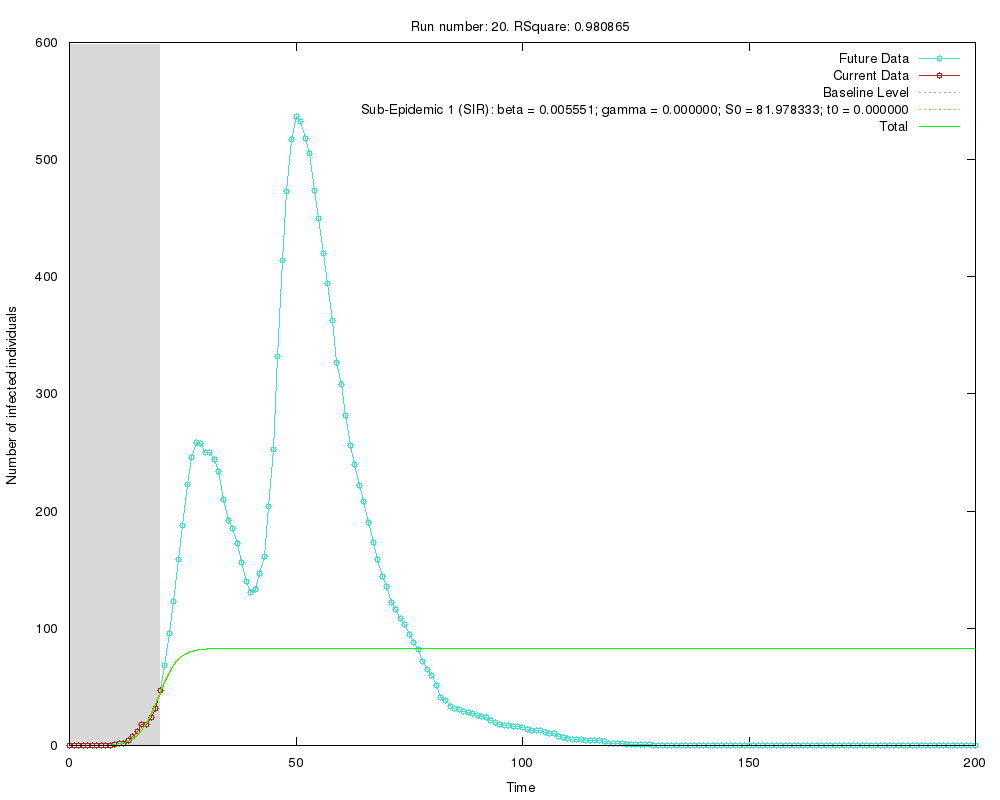
\includegraphics[width=8cm]{images/multi/sirsir1.png}
  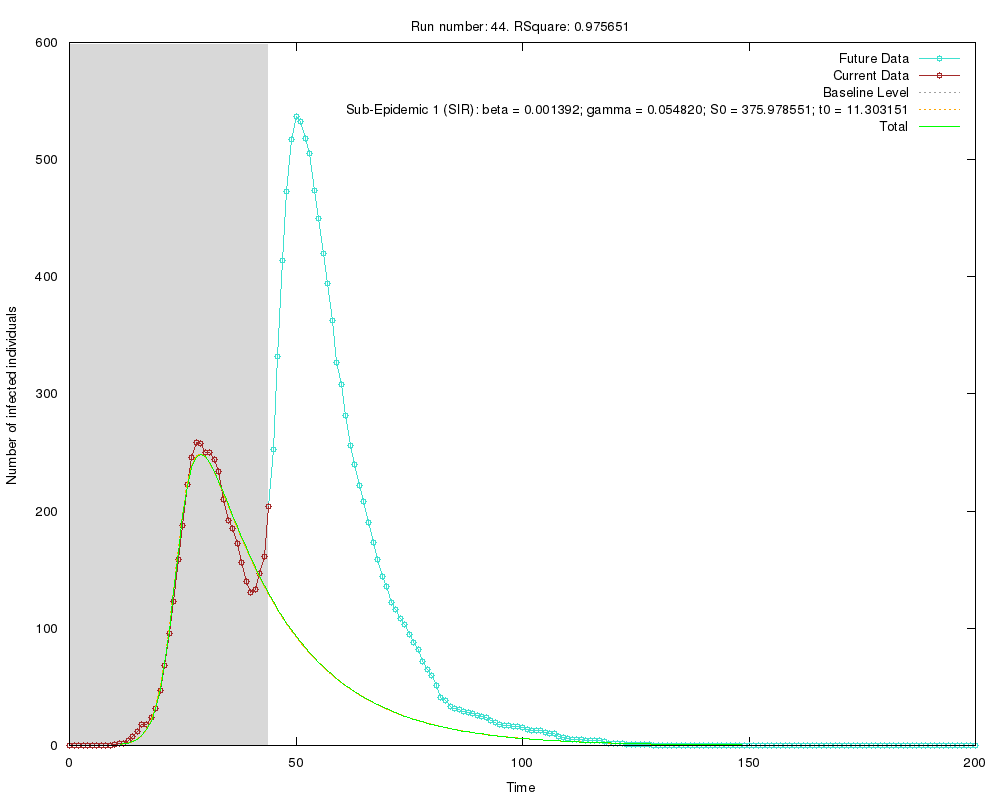
\includegraphics[width=8cm]{images/multi/sirsir2.png}
  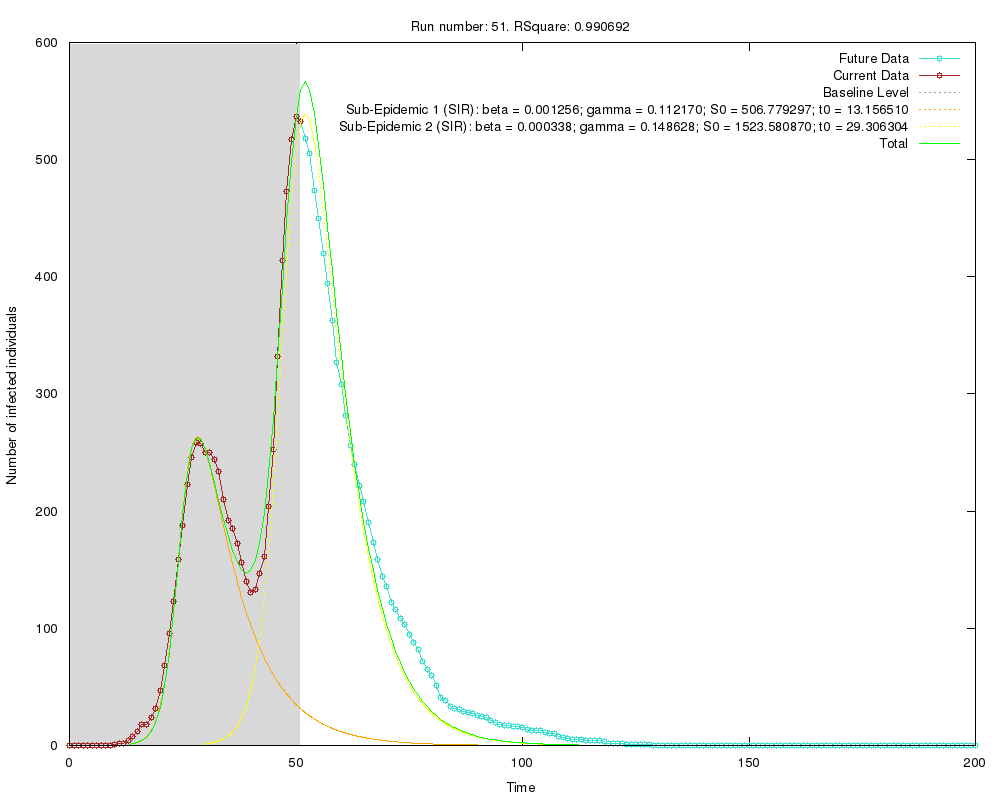
\includegraphics[width=8cm]{images/multi/sirsir3.png}
  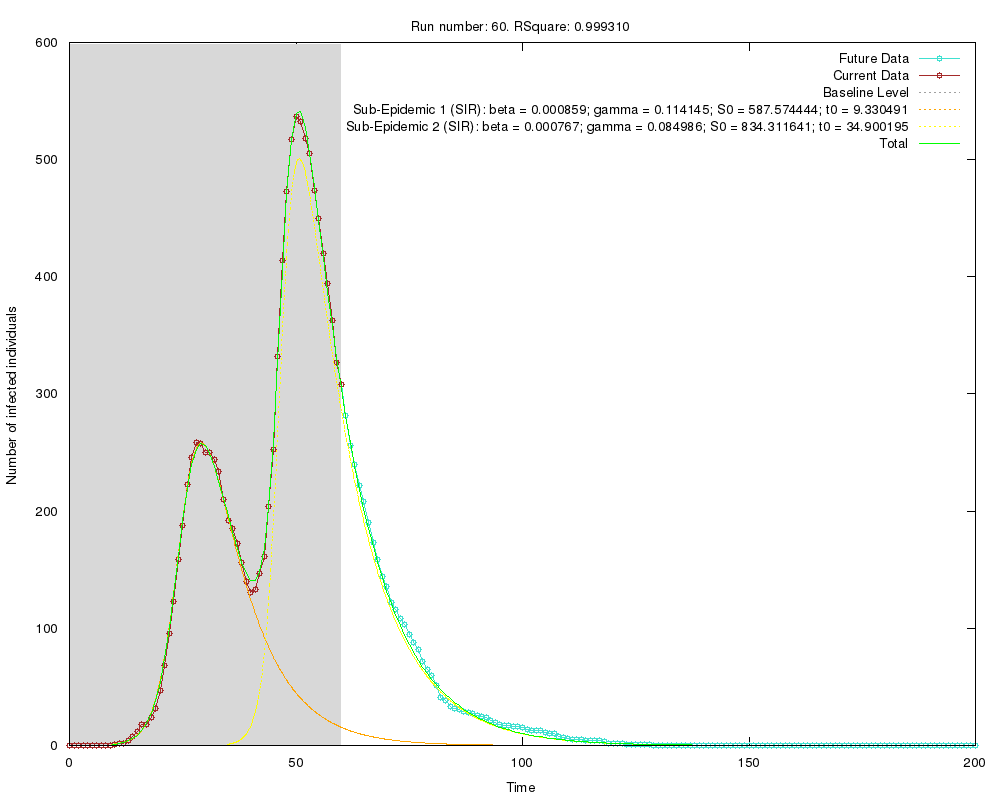
\includegraphics[width=8cm]{images/multi/sirsir4.png}
  \caption{Multiple epidemic fitting procedure on two overlapping SIR models}
\label{fig:sirsir1}
  \end{figure}
\end{centering}

As in the single epidemic fitting framework, a problem that
occasionally occured was that the the optimisation procedure
occasionally tended towards values far outside the range of realistic
values. For example, the optimisation makes $S_0$ very large as it
explores a particular local minimum. Furthermore, the inclusion of
$t_0$ as an additional parameter makes the optimisation procedure much
less stable, particularly when uncertainty in other model parameters
is high. This results in a model fit that is not quite as good as we
might hope, particularly when considering earlier sub epidemics. 


\subsection{Parameter Transformations and Bounding}
A potential way of limiting the space in which the Nelder-Mead
algorithm searches for parameters is to bound the parameters. As
discussed in section SECTION, it is often desirable to transform the model parameters into log space. Another potential transformation that may be applied is through the
use of the \emph{logistic} function. Originally studied in the context
of population growth, maps the parameter search space from between $0$ and $1$
to between $-\infty$ and $+\infty$. The function is
defined as:
\begin{equation}
logistic(x)=\frac{1}{1+e^{-x}}
\end{equation}
The inverse of the logistic function, the \emph{logit} function, can
therefore be used to map the search space of a parameter, \emph{p},
from between $-\infty$ and $+\infty$ to between $0$ and $1$. The logit
function is defined as:
\begin{equation}
logit(p) = log(\frac{p}{1-p})
\end{equation}
The logit function can be modifed to transform the search space from
between $0$ and $1$ to one between $0$ and $max$ as follows:
\begin{equation}
newLogit(x) = \frac{max}{1+e^{-x}}
\end{equation}
with the inverse defined as:
\begin{equation}
newLogistic(x)=log(\frac{x}{max-x})
\end{equation}

 The logic behind this modification can be expanded further to use the logistic function to provide lower bounds as well as upper bounds. As
$x\rightarrow +\infty$, $logit(x)\rightarrow 1$. Similarly, as
$x\rightarrow-\infty$, $logit(x)\rightarrow 0$. We can therefore modify
the logistic function as follows:
\begin{equation}
f(x) = \frac{x_{max}-x_{min}}{1+e^{-x}} + x_{min}
\end{equation}.

We can see that as $x\rightarrow +\infty$, $f(x)\rightarrow x_{max}$,
and as $x\rightarrow -\infty$, $f(x)\rightarrow x_{min}$. By limiting
the parameter search space to a predetermined range of expected
values, we ensure that the optimisation procedure does not get stuck
in a local minimum far away from the actual parameter values. However,
doing so requires us to make assumptions regarding where the real
parameter values might lie. Whilst a good model fit might be produced
within a provided range of parameter values, this fit might be sub
optimal compared to the model produced from a set of entirely
unexpected parameters. 

An alternative, simple approach to bounding parameter values in the
optimisation procedure is to modify the results returned by the
objective function. As the Nelder Mead algorithm transforms parameter
values with the aim of minimising the objective function, we can
direct the parameter search by ensuring that the objective function
returns high values when venturing into an undesirable parameter
space. For example, we can include a simple check of each parameter
with each call of the objective function; returning a high SSE value
if the parameter is outside our desired range. This method was
implemented initially; however, it appeared to result in the Nelder
Mead algorithm returning nonsense values more frequently as it failed
to identify any local minima. This is due to the fact that the
optimisation surface becomes much less smooth, as each check outside
of the specified bounds results in a sudden spike in function value.  

Using the above methodology, we initially add constant limits to $S_0$
and $t_0$; ensuring that $S_0$ stays within the range 100-15000, and
$t_0$ stays within the range of data (typically 0-200). Although this
did improve the stability of the fittnig procedure, it was found that
the range of possible $t_0$ values could be limited further. Rather
than using 0-200, we use a window of time around the detection
time. We use the detection time of the epidemic as the upper bound of
the transformation, and $t-40$ as the lower bound.

\section{Implementation Revision with Parameter Bounding}
Figure~\ref{fig:sirsir2} shows the results of the fitting procedure on
the same two overlapping SIR models usnig logitic bounding on $S_0$
and $t_0$. As in the previous implementation, the fitting procedure
maintains a high R Square value throughout, and accurately detects the
second epidemic. With an effective multiple SIR fitting framework, we
then attempt to consider the addition of an EXP model. As dicussed in
the context of single epidemic model fitting, we add the candidate
model that produces the best model fit in terms of \emph{AICc}
value. For $t_0$ bounding, we use a very narrow optimisation for the
EXP epidemic. Figure~\ref{fig:sirexp1} shows that the framework is able to
accurately detect and fit both the SIR and EXP model throughout the
fitting procedure.


\begin{centering}
\begin{figure}[h!]
  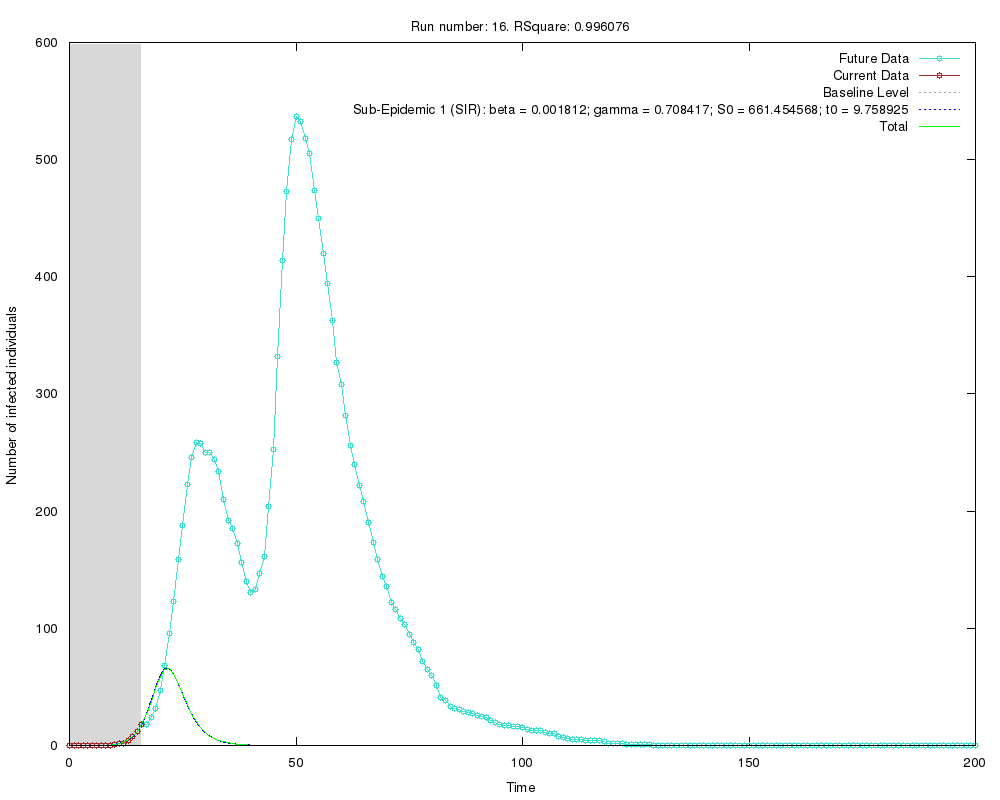
\includegraphics[width=8cm]{images/multi/sirsir6.png}
  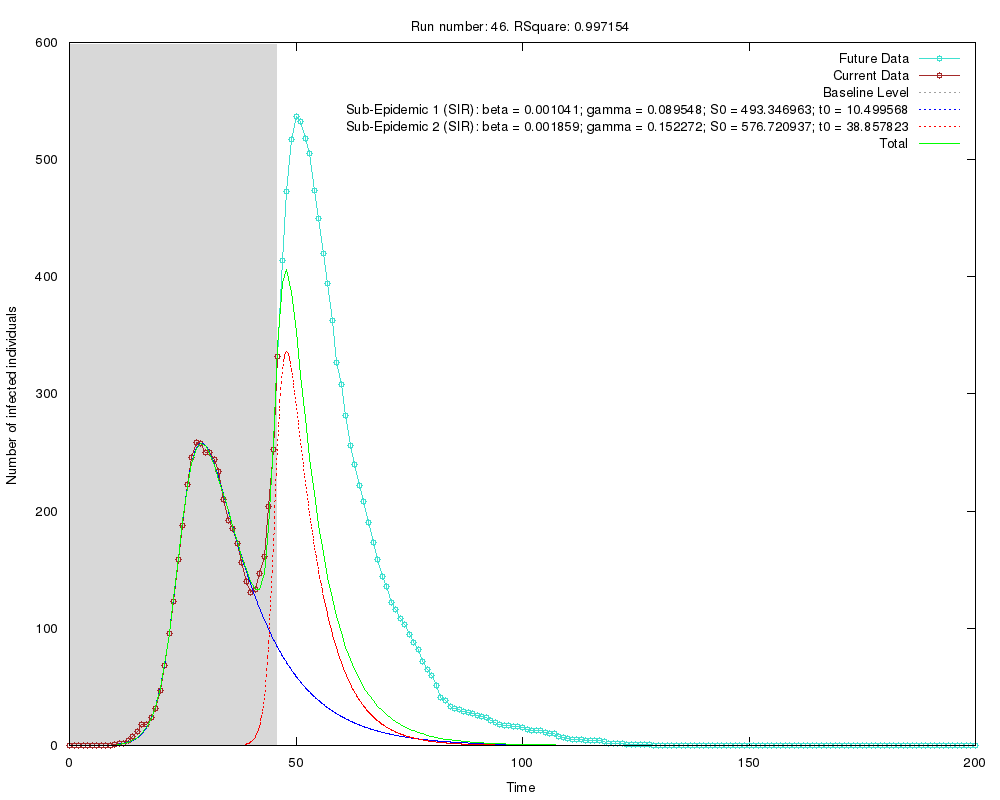
\includegraphics[width=8cm]{images/multi/sirsir7.png}
  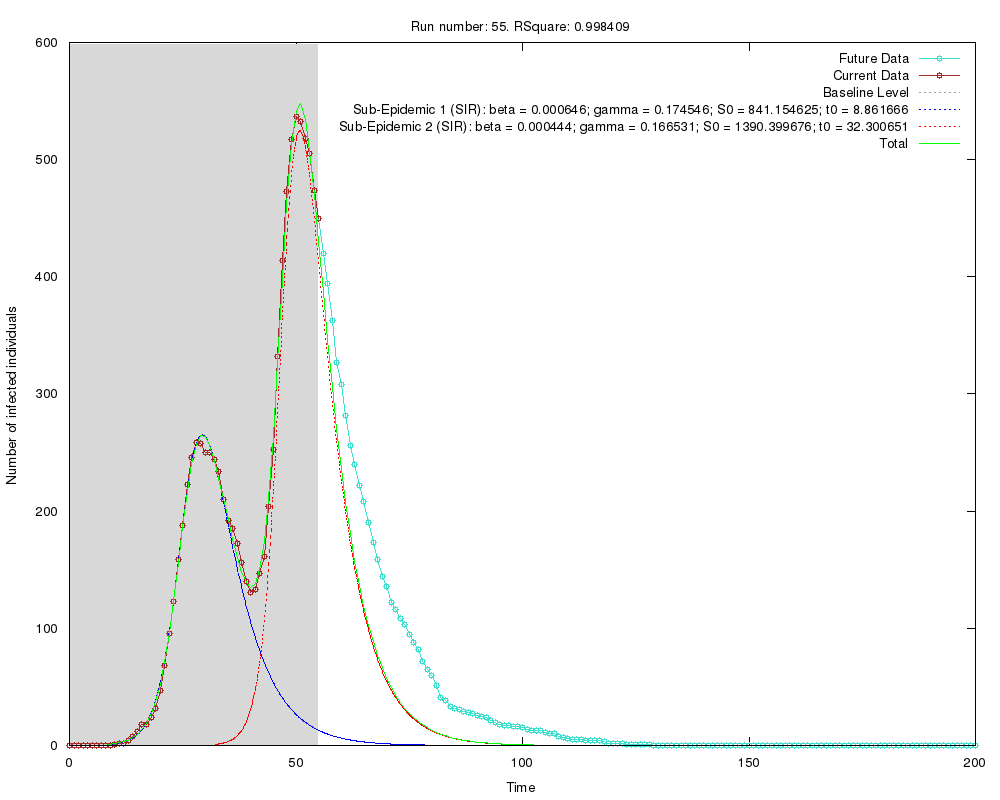
\includegraphics[width=8cm]{images/multi/sirsir8.png}
  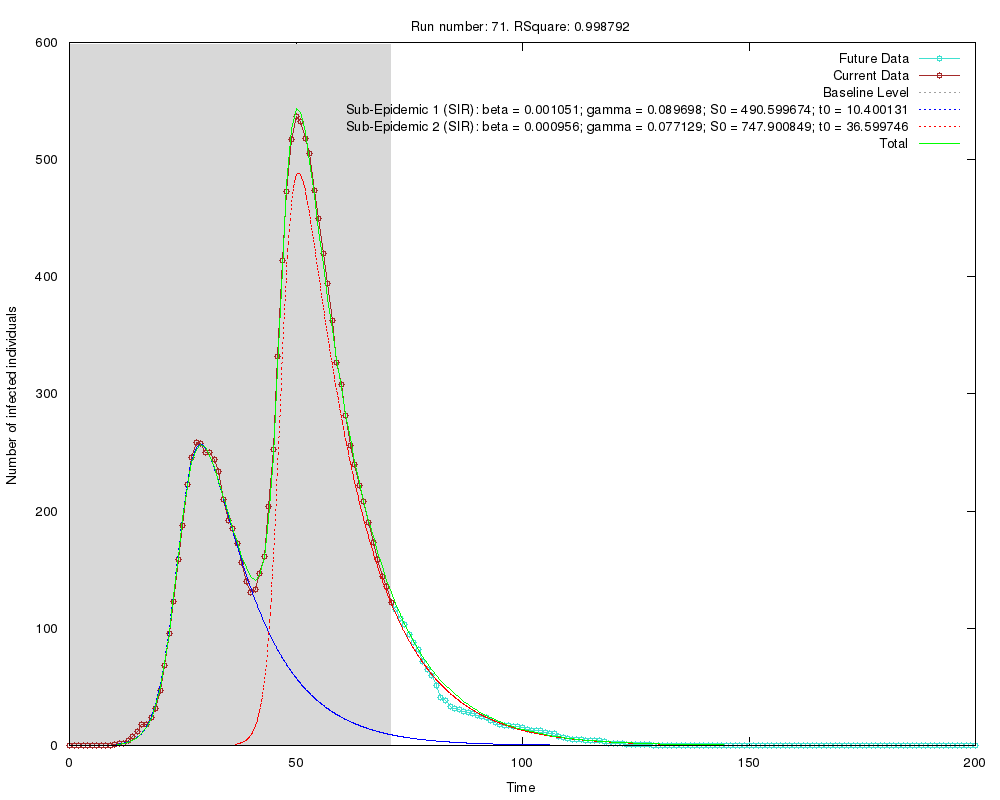
\includegraphics[width=8cm]{images/multi/sirsir9.png}
  \caption{Multiple epidemic fitting procedure on two overlapping SIR
    models with logistic bounding}
\label{fig:sirsir2}
  \end{figure}
\end{centering}


\begin{centering}
\begin{figure}[h!]
  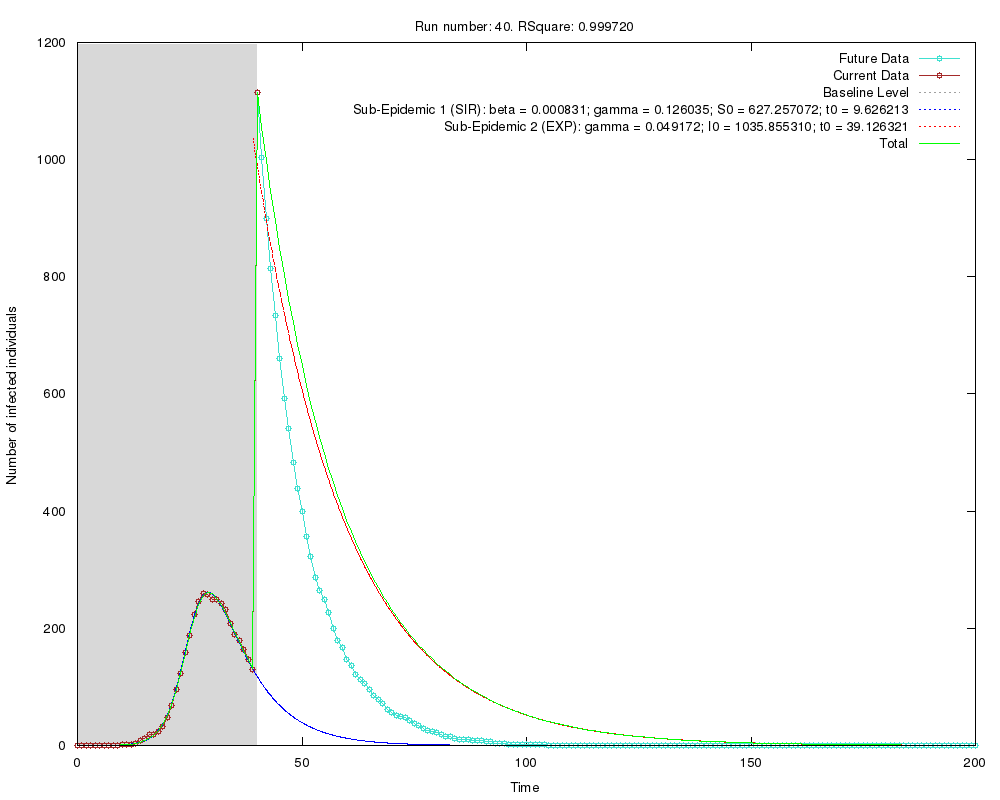
\includegraphics[width=8cm]{images/multi/sirexp1.png}
  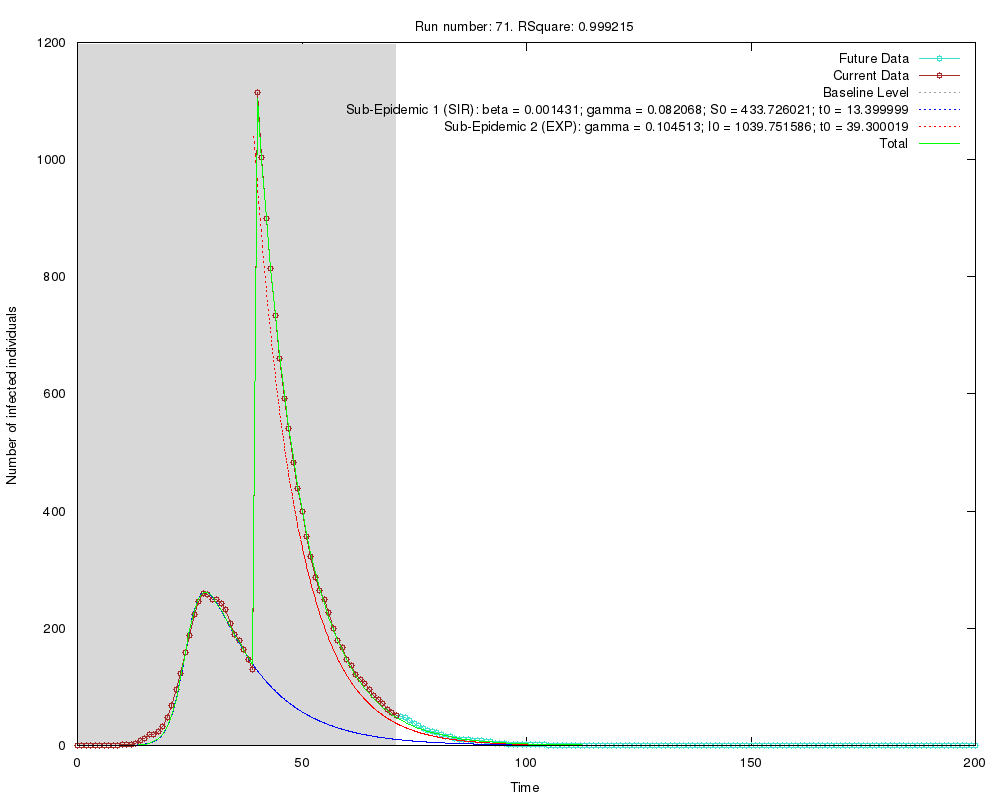
\includegraphics[width=8cm]{images/multi/sirexp2.png}
  \caption{Multiple epidemic fitting procedure on an SIR and EXP models with logistic bounding}
\label{fig:sirexp1}
  \end{figure}
\end{centering}

The true parameters used in figure~\ref{fig:sirexp1} are:

$SIR: beta = 0.001, gamma = 0.1, S_0 = 500, t_0 = 10$ \\
$EXP: gamma = 0.1, S_0 = 1000, t_0 = 40$


\section{Final Implementation}
With a multiple epidemic fitting framework implemented, we then went
on to test our epidemic fitting framework on real epidemic data. To
put the framework to the test, we firstly attempted to characterise
the viral internet sensation, ``Blurred Lines'' by Robin Thicke. To
speed up the fitting process, we only consider SIR and EXP models. We
use the number of \emph{BitTorrent} downloads between As
a first attempt, the model provided a reasonable fit to the data,
characterising the overall shape fairly well. However, as can be seen
in figure~\ref{fig:rt1}, there are a number of shortcomings in the
present approach:

\begin{enumerate}
  \item The characterisation of the first SIR epidemic worsens during
    the fitting procedure, particularly towards the end.
  \item The long term projection of the epidemic varies throughout the
    run. For example, whereas the first graph predicts that there will
    constantly be around 4000 infected individuals, the second graph
    predicts that the epidemic will eventually die out.
  \item The procedure is unable to pick up the epidemic peaks at
    around day 180 and day 220.
\end{enumerate}


\begin{centering}
\begin{figure}[h!]
  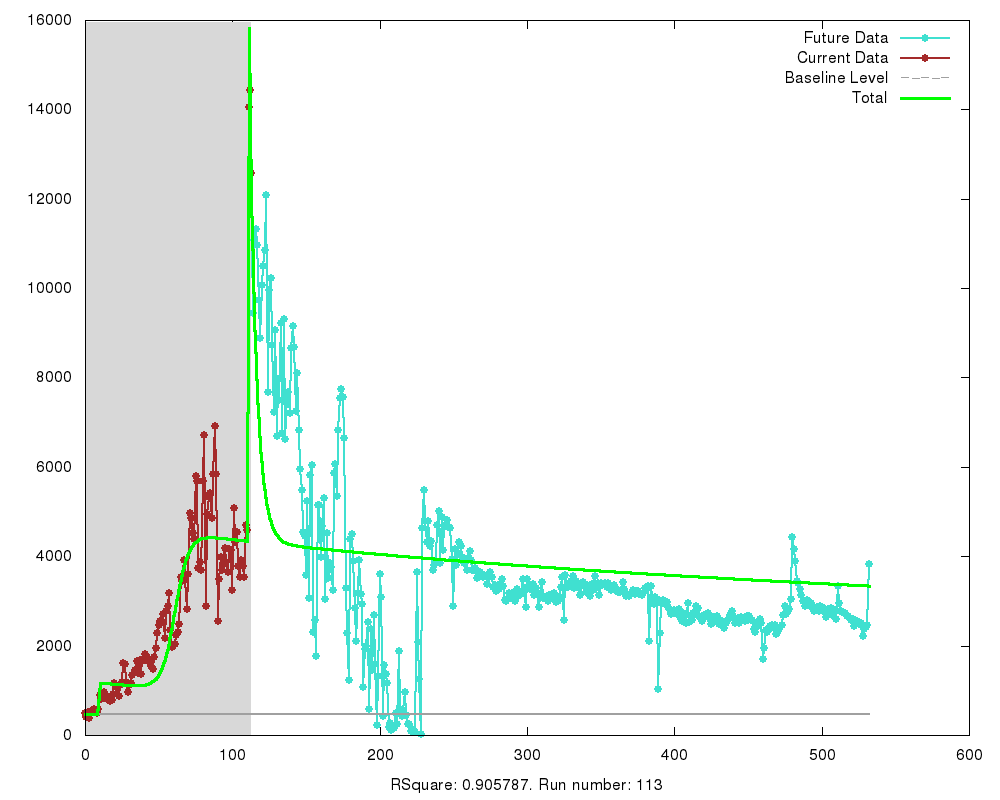
\includegraphics[width=8cm]{images/multi/badrt1.png}
  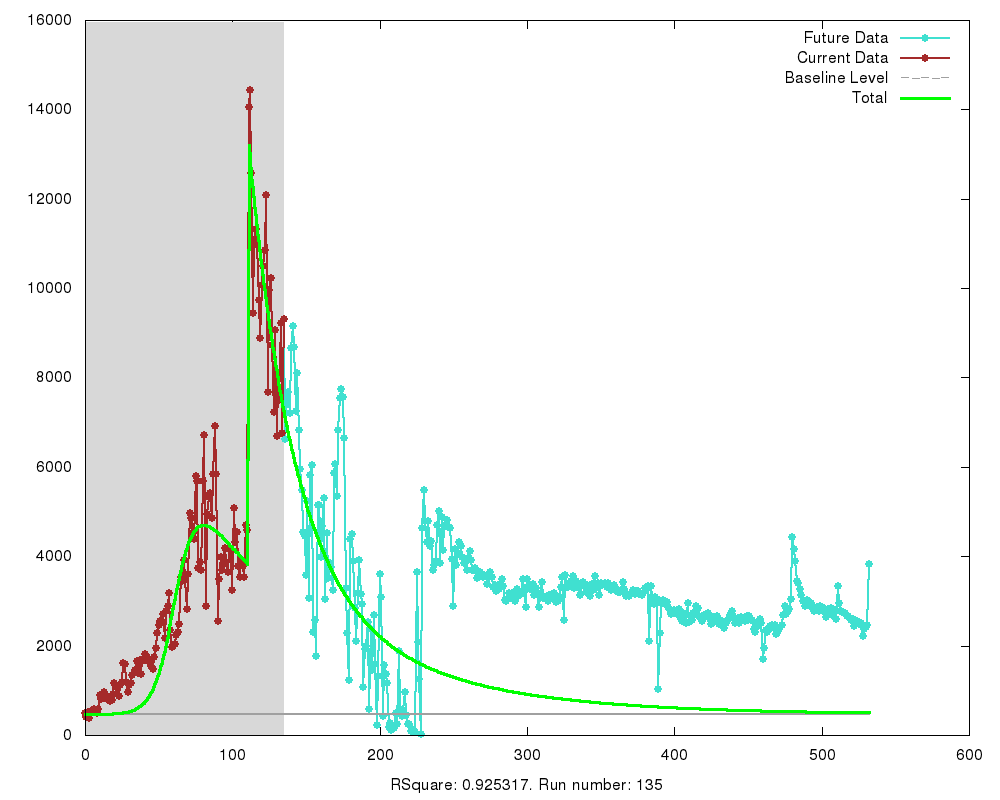
\includegraphics[width=8cm]{images/multi/badrt2.png}
  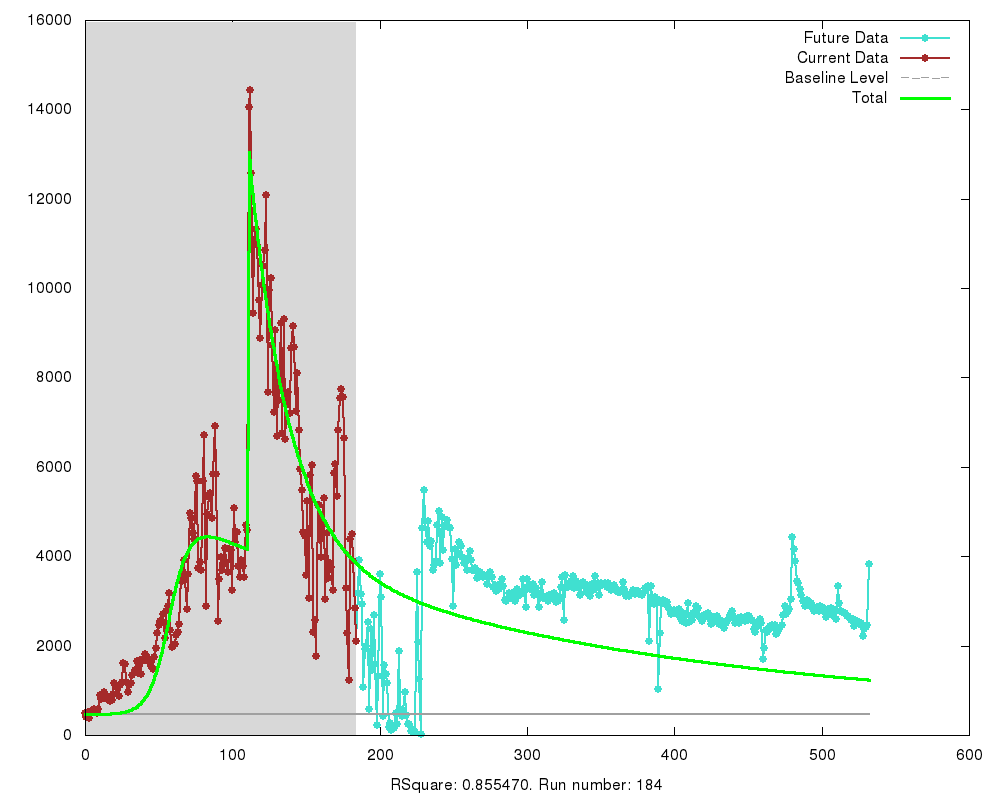
\includegraphics[width=8cm]{images/multi/badrt3.png}
  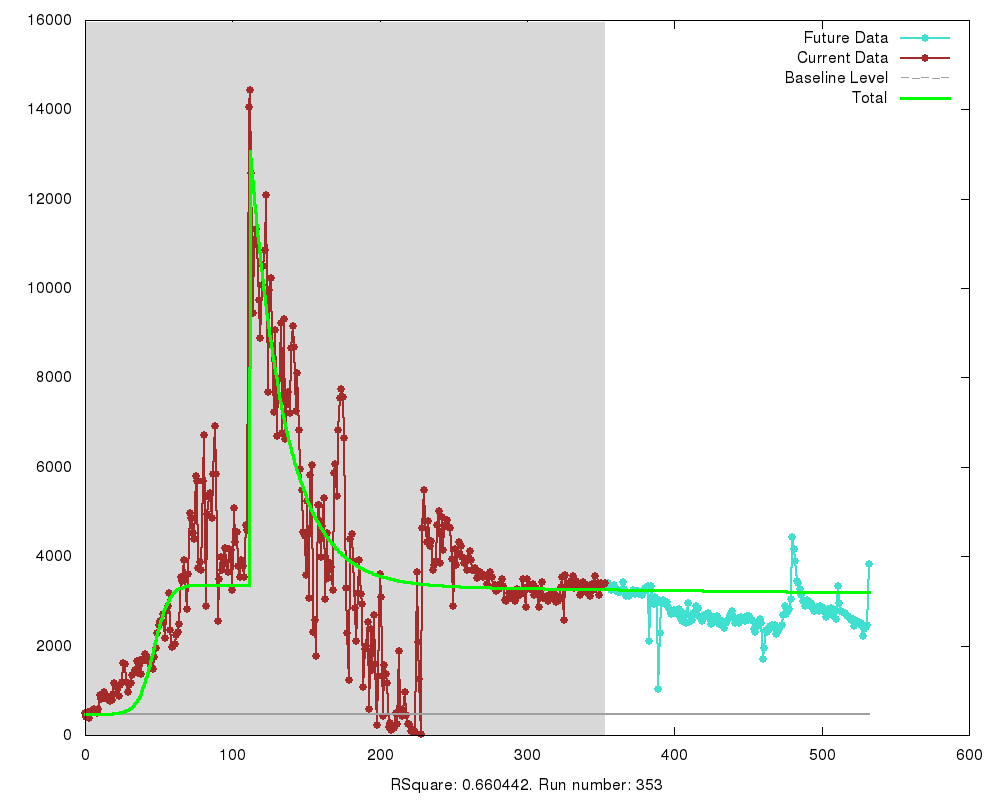
\includegraphics[width=8cm]{images/multi/badrt4.png}
  \caption{Multiple epidemic fitting procedure on the number of
    \emph{BitTorret} downloads of the song ``Blurred Lines'' by Robin
    Thicke. Number of downloads on the y-axis and day on the x-axis}
\label{fig:rt1}
  \end{figure}
\end{centering}

The main reasons for the this instability and inaccuracy can be
attributed to the following:

\begin{enumerate}
\item \textbf{Problem:} Not constraining the transition parameters (eg. beta and gamma)
  results in a number of optimisation runs that do not converge on a
  decent fitting solution. Furthermore, using a potential seed range
  of parameters that are too far from the correct value results in a
  number of unstable runs. For example, if the basic reproduction
  number, $R_0$ is less than one (where $R_0 =\frac{\beta}{\gamma}$),
  then the epidemic will not take off. It was found that seeding the
  optimisation with a high value of $S_0$ often produced non
  convergent runs.\\
  \textbf{Solution:} The seed times of the transition parameters
  should be adapted to ensure that they are within a reasonable
  range. Secondly, we can use the logistic transformation to bound
  these parameters within a sensible range. We also seed $S_0$ with a
  lower than expected value and allow the optimisation algorithm to
  `grow' the value.
\item \textbf{Problem:} The detection threshold for new epidemics is set too high. In
  the above run, we use a threshold R Square value for 0.8, which
  potentially allows for outlying data points to be ignored.\\
  \textbf{Solution:} The target R Square value is increased, and the
  distance to latest residual from the mean of the residuals is
  reduced to two standard deviations.
\item \textbf{Problem:} The time taken to run ten optimisations is
  longer than desirable.\\
  \textbf{Solution:} We investigated the effect of changing the
  scaling parameters in the Nelder-Mead algorithm itself. We initially
  used parameter values of 1.0, 1.0, 0.5 and 0.5 for reflection,
  expansion, contraction and secondary contraction respectively. The
  expansion parameter is particularly troublesome, as it currently
  does not stretch the simplex towards the best vertex. We therefore
  changed these values to 1.1, 1.5, 0.4 and 0.4 respectively, which
  resulted in a significant decrease in optimisation time.
\end{enumerate}

Following the above modifications, the framework was rerun on the
``Blurred Lines'' download data as shown in
figure~\ref{fig:goodrt}. Note that the number of data points is
reduced by taking every fourth data point to reduce run time.

\begin{centering}
\begin{figure}[h!]
  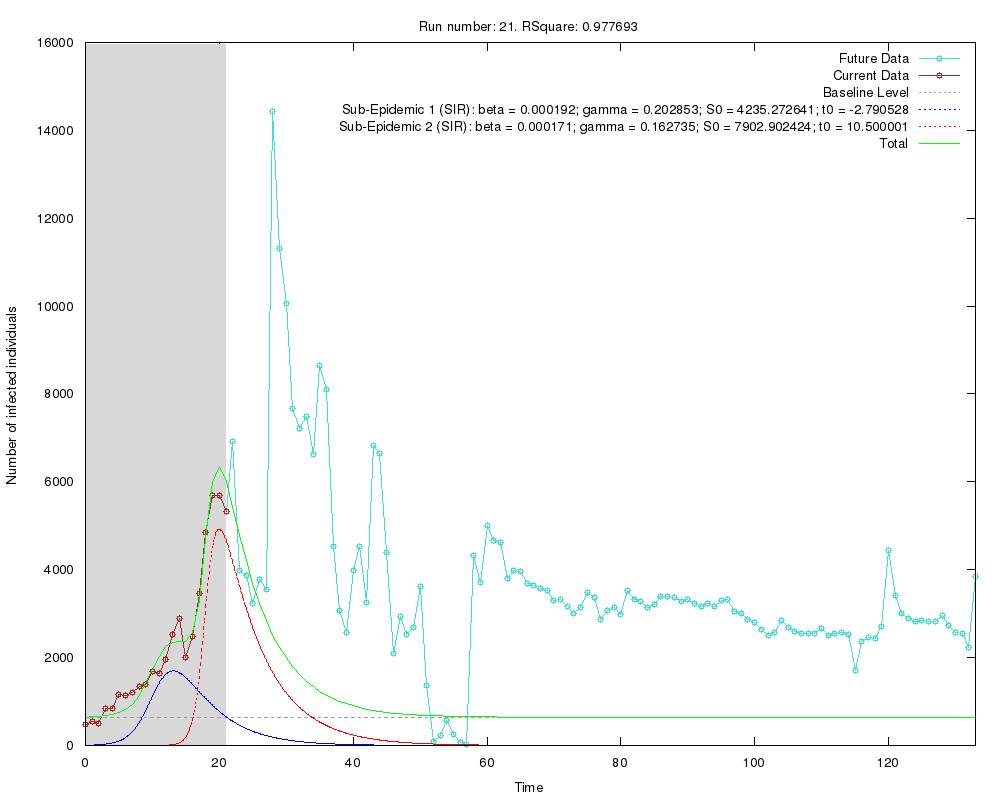
\includegraphics[width=8cm]{images/multi/goodrt1.png}
  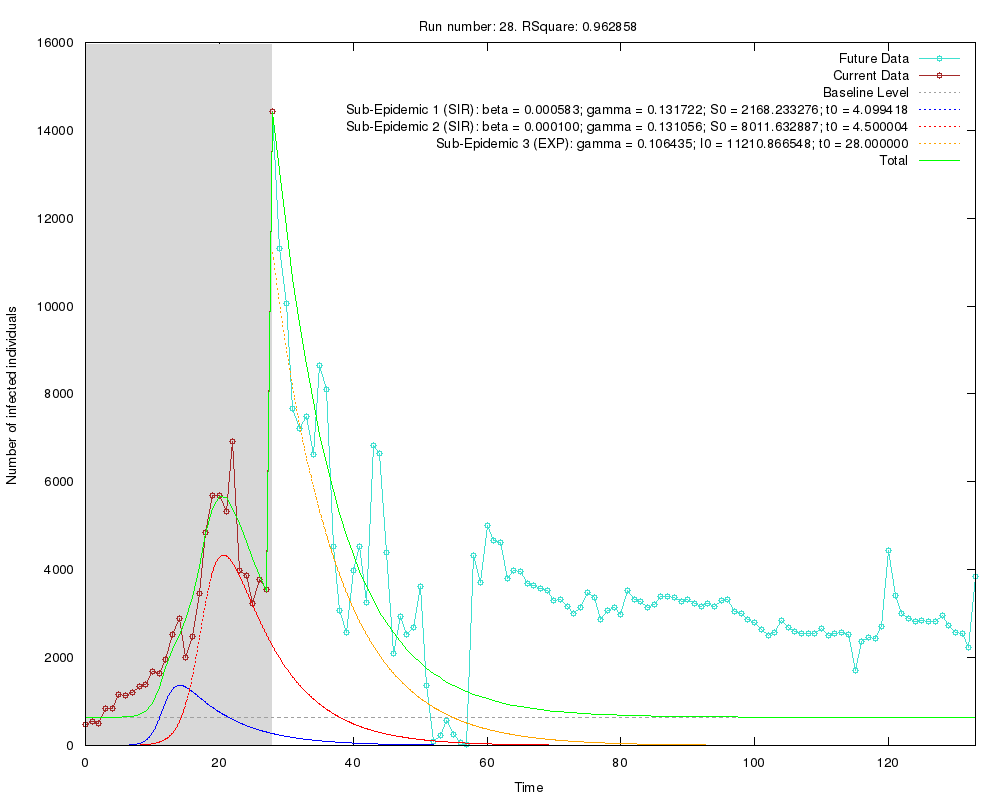
\includegraphics[width=8cm]{images/multi/goodrt2.png}
  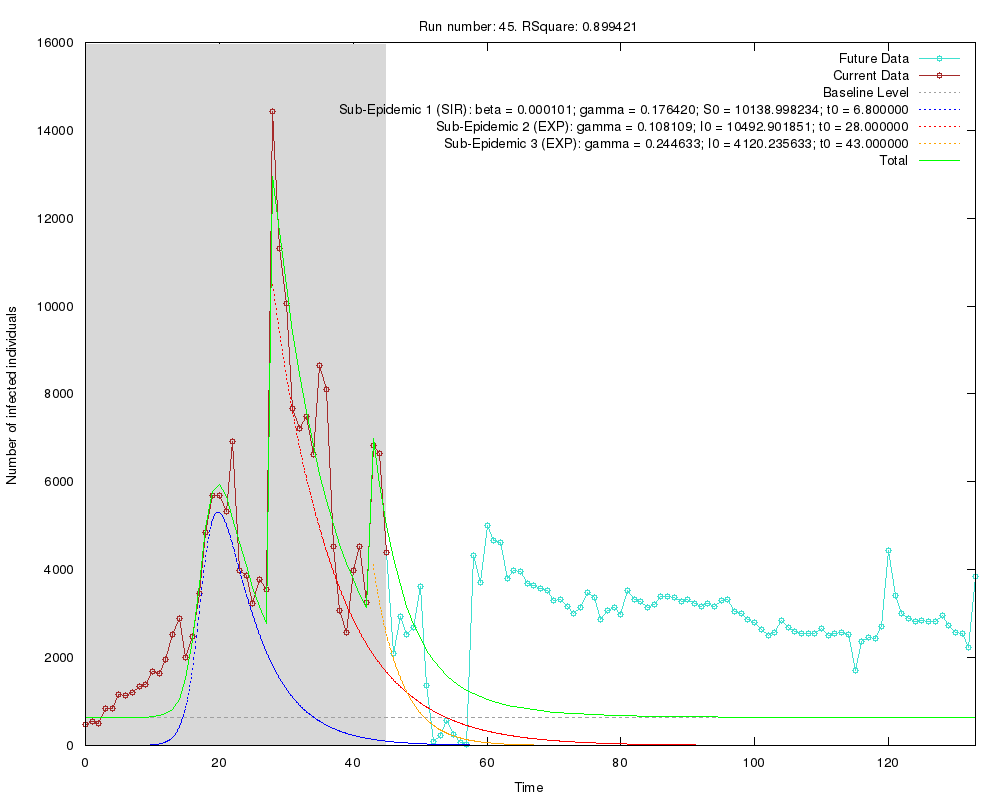
\includegraphics[width=8cm]{images/multi/goodrt3.png}
  \caption{Second multiple epidemic fitting procedure on ``Blurred
    Lines'' download data using additional logistic binding and
    modified Nelder-Mead algorithm }
\label{fig:goodrt}
  \end{figure}
\end{centering}

The updated implementation provides a much better fit throughout the
course of the run, and accurately locates the start of constituent
epidemics. Interestingly, these sub epidemics can be ascribed to real
world events that resulted in the sudden expose of ``Blurred
Lines''. The initial SIR shaped epidemic seems to be a result of the
initial video upload in March 2013. The second, larger spike epidemic
immediately follows the exposure of Robin Thicke on the US television
show, ``Jimmy Kimmel Live''. Another epidemic is detected at around
day 200, which coincides with the live performance of ``Blurred
Lines'' on the 2013 ``MTV Video Music Awards''. Finally, the final
epidemic at around day 250 immediately follows Robin Thicke's appearance on the TV show ``X Factor''.  



\section{Implementation Summary}
The model fitting framework proposed in figure~\ref{fig:uml} was
adapted to form the final synthedemic fitting framework. The flow of
control is summarised as follows:

\begin{enumerate}
\item An instance of the Datahandler class imports the desired
  epidemic data from a .csv file into a vector.
\item The Datahandler object begins the iterative fitting procedure
  with a target R Square value, as shown in \ref{fig:realtime}.
\item The fitting procedure starts with no epidemics, and attempts to
  find an optimal synthedemic model fit to the currently available
  data at each time point. This is done by passing the objective
  function in \ref{fig:objective} to an instance of the ``Nelder
  Mead'' class.
\item To prevent overfitting, the framework also attempts to optimise
  all possible $k-1$ epidemic combinations at each time point. If the
  resulting R Square value is above the threshold, the epidemic is
  permanently removed.
\item If the R Square value is below the desired threshold and a new
  epidemic outbreak has been detected, we
  consider adding each candidate model. We then choose to add the
  model with the lowest AICc score.
\item At the end of each time point, we plot the results of the
  optimisation and reset all temporary parameters.
\end{enumerate}

The Datahandler class stores a number of attributes that are used in the
optimisation procedure. For example, the currently avaiable data, the current best
fitting model and a vector of Epidemic objects. The reasoning behind
storing so many variables as properties rather than declaring them
locally is to speed up the optimisation procedure. The presented
implementation also uses logistic bounding on all parameters within a
sensible range to reduce the chance of the optimisation algorithm from
getting stuck in a bad local minima. The start time of each epidemic,
$t_0$ is also included in the optimisation procedure. By using
different bounds for each Epidemic sub class, we are able to limit the
parameter search space for each sub epidemic depending on the epidemic
type.

\begin{algorithm}
  \captionof{figure}{Synthedemic Fitting Framework Function}
  \begin{algorithmic}
    \Function{realtime\_model\_fit}{targetRSq, data} 
    \State //\emph{Begin the iterative procedure}
    \For{i = 0 to length(data)}
    \State //\emph{Get currently available data}
    \State availableData = data[1:i]\\
    \State //\emph{Optimise current set of $k$ epidemics to data}
    \State (optimParams, modelResults, RSquare, AICc) =
      optimiseEpidemics(availableData, epidemics)
      \\
      \If{RSquare \textgreater targetRSq}
      \For{j = 0 to length(epidemics)}
        \State tempEpidemics = fewer\_epidemics(j);\\
        \State //\emph{Optimise for $k-1$ epidemics}
        \State (tempParams, tempModel, tempRSquare, tempAICc) =
        optimiseEpidemics(availableData, tempEpidemics);\\
        \State //\emph{If fit sufficient, track this epidemic for removal}
        \If{tempAICc \textless AICc \& tempRSquare \textgreater
          targetRSq}
        \State //\emph{Store results for $k-1$ epidemics}
        \EndIf
        \State tempEpidemics = epidemics;
        \EndFor
        \EndIf
      \State remove\_epidemic(toRemove);
      \\
      \State //\emph{Check residuals for new outbreak}
      \State residuals = get\_residuals(availableData, modelResults);
      \State newEpidemic = check\_for\_epidemic();
   \\ 
   \State //\emph{If an epidemic was detected and the current fit is
     insufficient, attempt to add an epidemic}
   \If{newEpidemic != true \& RSquare \textless targetRSquare}
   \State tempEpidemics = epidemics;
   \\
   \State //\emph{Check the addition of each candidate model}
   \For{j = 0 to length(candidateModels)}
   \State tempEpi = newEpidemic(candidateModels[j]);
   \State tempEpidemics.push\_back(tempEpidemic);\\
   \State //\emph{Optimise for $k+1$ epidemics}
   \State (tempParams, tempResults, tempRSquare, tempAICc) = optimiseEpidemics(availableData, tempEpidemics);
   \If{tempAICc \textless AICc \& tempRSquare \textgreater
     targetRSq}
   \State toAdd = tempEpi;
   \State //\emph{Store results for $k+1$ epidemics}
   \EndIf
   \EndFor
   \EndIf\\
   \If{toAdd != NULL} epidemics.push\_back(toAdd); \EndIf
   \EndFor
   \EndFunction
  \end{algorithmic}
  \label{fig:realtime}
  \end{algorithm}

Note that at each time point that an epidemic is detected, we test the
model fit when each sub epidemic is removed. An alternative, simpler
approach would be to only consider removing the last epidemic at each
time point. Although this would improve the speed of the fitting
procedure, we risk leaving in superfluous sub epidemics from early on
in the fitting procedure. Including $t_0$ in the optimisation also
improves the ability of the remaining sub epidemics to compensate for
dropping an epidemic.

\begin{algorithm}
  \captionof{figure}{Epidemic Optimisation Function}
  \begin{algorithmic}
    \Function{optimise\_epidemics}{epidemics, availableData}
    \If{length(epidemics) == 0}
    \State model = baseline\_model(availableData);
    \State RSquare = calculate\_RSquare(model, availableData);
    \State AICc = calculate\_AICc(model, availableData);
    \State finalParams = ();
    \Else
    \State//\emph{Perform 10 random fits and choose best fitting run}
    \For{i = 0 to 10}
    \State seedParams = generate\_seed\_parameters();
    \State logit\_transform\_parameters(seedParams);
    \State (tempParams, tempSSE) = neldermead\_optim(*ode\_solve\_sse, seedParams);
    \If{tempSSE \textless SSE}
    \State SSE = tempSSE;
    \State finalParams = tempParams;
    \EndIf
    \EndFor
    \State model = ode\_solve(finalParams);
    \State AICc = calculate\_AICc(model, availableData);
    \State RSquare = calculate\_RSquare(model, availableData);
    \Return (finalParams, model, RSquare, AICc);
    \EndIf
    \EndFunction
  \end{algorithmic}
\label{fig:optimise}
\end{algorithm}


\begin{algorithm}
  \captionof{figure}{ODE Solving Function}
  \begin{algorithmic}
    \Function{ode\_solve}{parameters}
    \State total\_model = empty\_model
    \State total\_model = combine\_vectors(total\_model,baseline\_model);
    \State logistic\_transform\_parameters(parameters);
    \For{i = 0 to length(epidemics)}
    \State temp\_model = epidemics[i].ode\_solve(parameters);
    \State total\_model = combine\_vectors(total\_model,
    temp\_model);
    \EndFor
    \Return calculate\_sse(total\_model,current\_data);
    \EndFunction
    \end{algorithmic}
  \label{fig:objective}
\end{algorithm}
    
 Each Epidemic object also has its own set of ODEs. By calling the ``ode\_solve''
function for each Epidemic object separately, we are able to easily
include additional epidemic types without having to change the
optimisation framework. It should also be noted that different
candidate models require different logistic bounds. For example,
whereas the beta value of a typical \emph{SIR} model might lie in the
range of 0.0005 to 0.005, a typical beta value for an \emph{irSIR}
model is between 0.00001 and 0.0001. Again, by including using an
object oriented approach, we are able to bind the parameters of each
sub epidemic depending on its type. A final observation regarding
figure~\ref{fig:objective} is that it can easily be modified to return
the calculated model rather than the SSE value.

 
